%\externaldocument[-f]{c2_foundations}
%\externaldocument[-f]{c3_simulation_experiments}
\chapter{Results}
\label{chap:4}
The experimental results are presented in this chapter. First, the parameters for the variables introduced in \cref{chap:3} are given. Then a sample of simulated trajectories are shown as an example. Finally, the inference results are presented.

\section{Configurations}
The configurations given below are used for the results presented in the following sections, if not specified otherwise.
\begin{itemize}
	\item Gamma priors for parent dynamics such that $ \textbf{Q}_{i} \sim Gam(\boldsymbol{\alpha}^i, \boldsymbol{\beta}^i)$ for $i \in \left\lbrace 1,2\right\rbrace $, and $ \boldsymbol{\alpha} = [\alpha_0, \alpha_1] $ and $ \boldsymbol{\beta} = [\beta_0, \beta_1] $
	\begin{align}
	\boldsymbol{\alpha}^1 = [5,10] &\quad \boldsymbol{\beta}^1 = [5,20] \\
	\boldsymbol{\alpha}^2 = [10,10] &\quad \boldsymbol{\beta}^2 = [10,5]
	\label{eq:gamma_params}
	\end{align}
	\item Transition intensity matrices of $ X_1 $ and $ X_2 $ sampled from priors given above
	\begin{align}
	\textbf{Q}_1 &= 
	\begin{bmatrix}
	-1.117 & 1.117 \\
	0.836 &  -0.836
	\end{bmatrix} \\
	\textbf{Q}_2 &= 
	\begin{bmatrix}
	-1.1 & 1.1 \\
	2.445 &  -2.445
	\end{bmatrix}
	\end{align}
	\item State space, $ \textit{S} = \rchi_{P} = \left\lbrace (0, 0), (0, 1), (1, 0),(1, 1)\right\rbrace $
	\item Observation space, $ \mathcal{Y} = \left\lbrace 0, 1, 2 \right\rbrace $
	\item Action space, $ \textit{A} = \left\lbrace a_{0}, a_{1} \right\rbrace = \left\lbrace 0, 1\right\rbrace $
	\item The set of transition intensity matrices of $ X_3 $
	\begin{align}
	\textbf{\textit{Q}}_3 = \left\lbrace \textbf{Q}_{3\mid a_{0}}, \textbf{Q}_{3\mid a_{1}} \right\rbrace = \left\lbrace 
	\begin{bmatrix}
	-0.5 & 0.5 \\
	2 &  -2
	\end{bmatrix}, 
	\begin{bmatrix}
	-3 & 3 \\
	0.02 &  -0.02
	\end{bmatrix} 
	\right\rbrace 
	\end{align}
	\item Number of particles, $ N = 200 $
	\item Weights of the policy introduced in \autoref{eq:policy}, $ \textbf{w} = [0.02, 0.833, 0.778, 0.87] $
\end{itemize}

\section{Simulation}
%It should be noted that the initial states are drawn from disrete uniform distribution.
%\begin{equation}
%\textbf{X}(0) \sim \mathcal{U} \left\lbrace 0, 1\right\rbrace 
%\end{equation}
%\begin{figure}[H]
%	\begin{center}
%		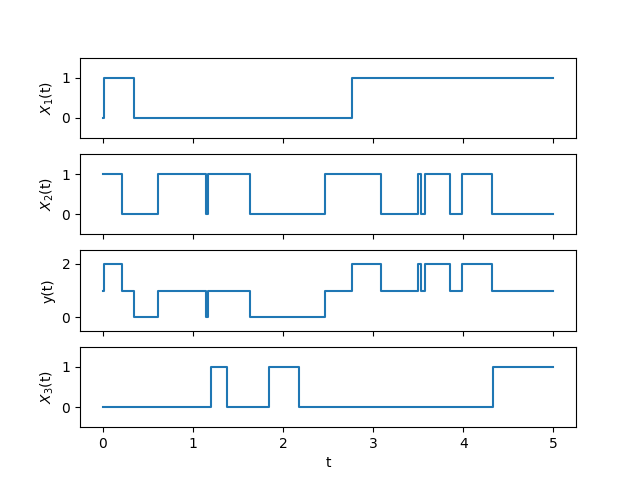
\includegraphics[width=.60\textwidth]{figures/traj}
%		\caption{Sampled trajectories}
%		\label{fig:simulation}
%	\end{center}
%\end{figure}
%\begin{figure}[H]
%	\begin{center}
%		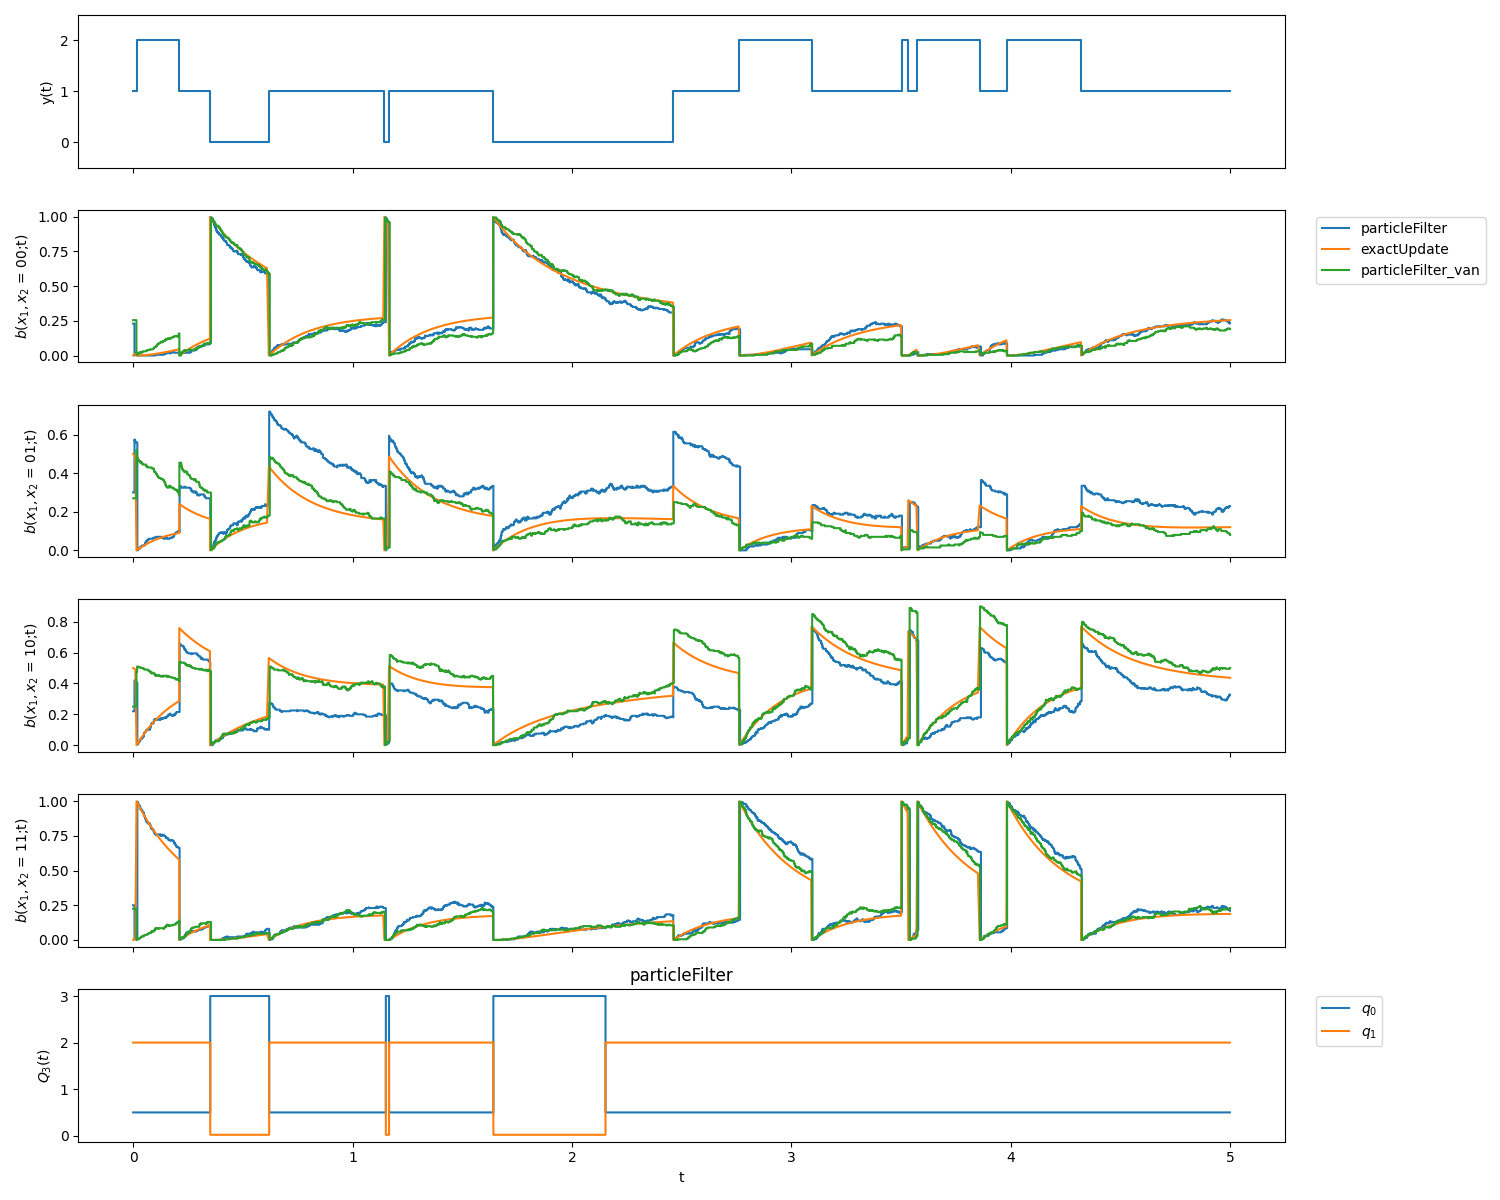
\includegraphics[width=.60\textwidth]{figures/b_q_traj}
%		\caption{Belief state and $ Q_3 $ trajectories}
%		\label{fig:b_q_traj}
%	\end{center}
%\end{figure}

\section{Inference of Observation Model}
%\subsection{Maximum Likelihood Estimation}
%\subsubsection{Equivalence Classes}
%
%$\psi_{true} =
%\begin{bmatrix} \vspace{-2pt}
%	1 & 0 & 0 \\  \vspace{-2pt}
%	0 & 1 & 0 \\  \vspace{-2pt}
%	0 & 1 & 0 \\  \vspace{-1pt}
%	0 & 0 & 1
%\end{bmatrix}$
%$\psi_{0} =
%\begin{bmatrix} \vspace{-2pt}
%1 & 0 & 0 \\  \vspace{-2pt}
%0 & 1 & 0 \\  \vspace{-2pt}
%0 & 1 & 0 \\  \vspace{-1pt}
%0 & 0 & 1
%\end{bmatrix}, 
%\psi_{1} =
%\begin{bmatrix} \vspace{-2pt}
%0 & 0 & 1 \\  \vspace{-2pt}
%0 & 1 & 0 \\  \vspace{-2pt}
%1 & 0 & 0 \\  \vspace{-1pt}
%0 & 0 & 1 
%\end{bmatrix},
%\psi_{2} =
%\begin{bmatrix} \vspace{-2pt}
%0 & 0 & 1 \\  \vspace{-2pt}
%1 & 0 & 0 \\  \vspace{-2pt}
%0 & 0 & 1 \\  \vspace{-1pt}
%0 & 1 & 0  
%\end{bmatrix}$
%
%\subsection{Maximum Likelihood Classification}
%\begin{figure}[htb]
%	\begin{subfigure}{.33\textwidth}
%		\centering
%		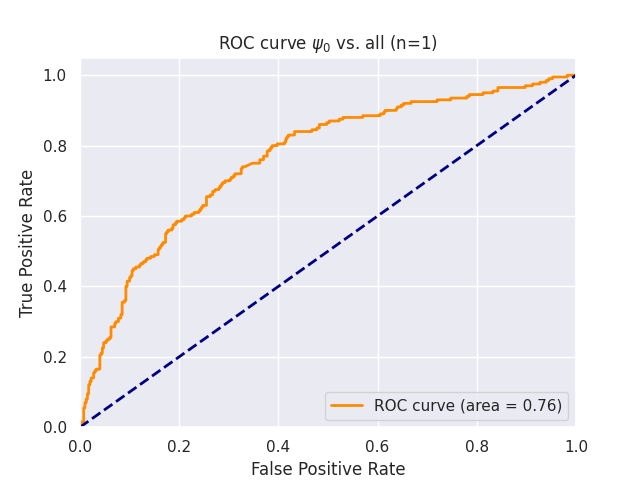
\includegraphics[width=1\linewidth]{figures/AUROC_600samples_class0_llh_n1}
%		\caption{}
%		\label{fig:sfig1}
%	\end{subfigure}%
%	\begin{subfigure}{.33\textwidth}
%		\centering
%		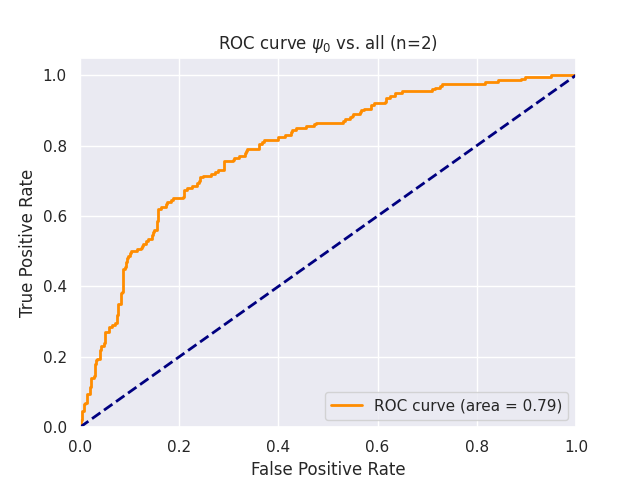
\includegraphics[width=1\linewidth]{figures/AUROC_600samples_class0_llh_n2}
%		\caption{}
%		\label{fig:sfig2}
%	\end{subfigure}
%	\begin{subfigure}{.33\textwidth}
%		\centering
%		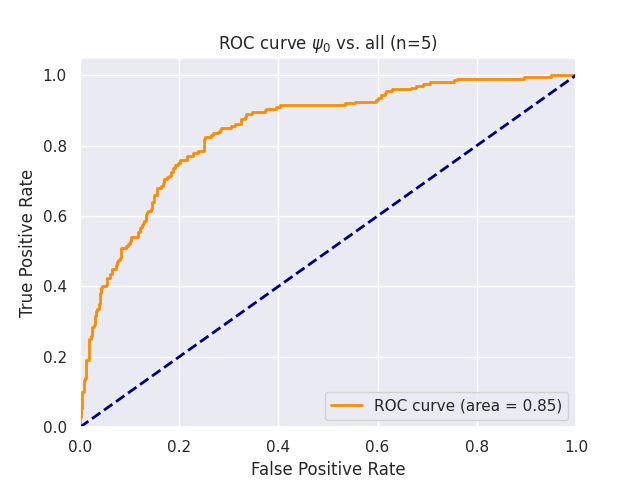
\includegraphics[width=1\linewidth]{figures/AUROC_600samples_class0_llh_n5}
%		\caption{}
%		\label{fig:sfig2}
%	\end{subfigure}\\
%	\begin{subfigure}{.33\textwidth}
%		\centering
%		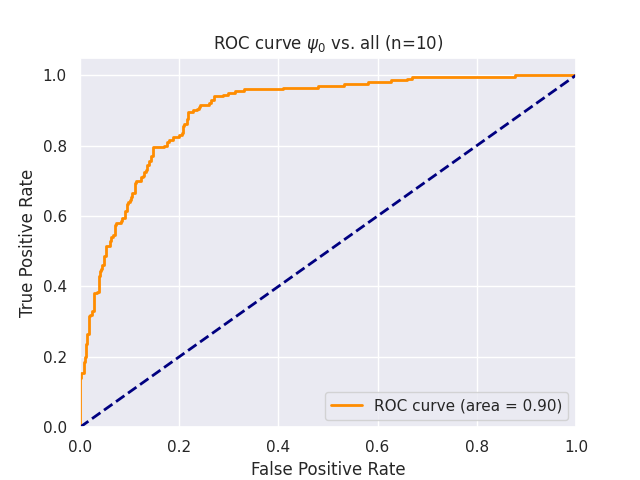
\includegraphics[width=1\linewidth]{figures/AUROC_600samples_class0_llh_n10}
%		\caption{}
%		\label{fig:sfig1}
%	\end{subfigure}%
%	\begin{subfigure}{.33\textwidth}
%		\centering
%		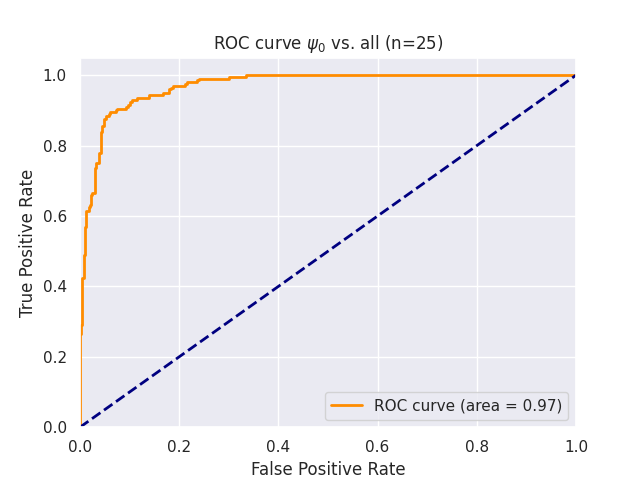
\includegraphics[width=1\linewidth]{figures/AUROC_600samples_class0_llh_n25}
%		\caption{}
%		\label{fig:sfig2}
%	\end{subfigure}
%	\begin{subfigure}{.33\textwidth}
%		\centering
%		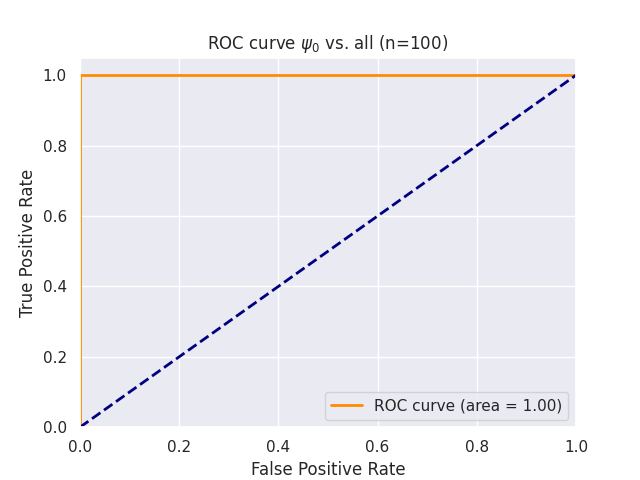
\includegraphics[width=1\linewidth]{figures/AUROC_600samples_class0_llh_n100}
%		\caption{}
%		\label{fig:sfig2}
%	\end{subfigure}
%	\caption{plots of....}
%	\label{fig:fig}
%\end{figure}
%\begin{figure}[htb]
%	\begin{center}
%		\includegraphics[width=.9\textwidth]{figures/all_particlefilter}
%		\caption{plot of...}
%		\label{fig:traj_}
%	\end{center}
%\end{figure}
